
%%%%%%%%%%%%%%%%%%%%%%%%%%%%%%%%%%%%%%%%%%%%%%%%%%%%%%
\chapter{Theoretical background}
%%%%%%%%%%%%%%%%%%%%%%%%%%%%%%%%%%%%%%%%%%%%%%%%%%%%%%


In this section I will organize and discuss the main theoretical building blocks that will be required to overcome the challenges previously identified and bring answers to the inquires this dissertation have raised. \par





\begin{figure}[h!]
    \centering
    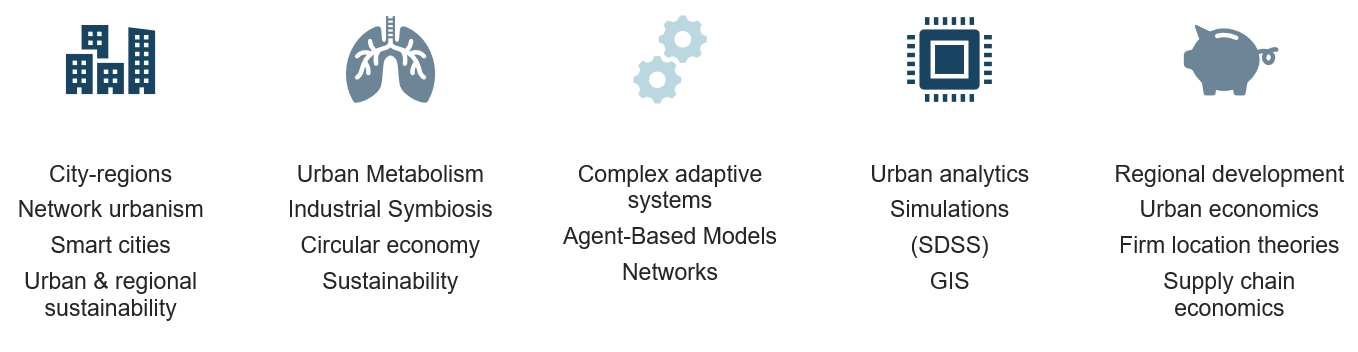
\includegraphics[width=0.8\textwidth]{sections/asset/theo.PNG}
    \caption{Theoretical background. Main research domains}
    \label{fig:theo}
\end{figure}





In order to make a substantial contribution as an interdisciplinary research and avoid falling in superficial -or wrong – analysis it would be crucial to become aware and build knowledge in different domains. Consequently, it is important to have a clear conceptual idea of the different definitions, assumptions, perspectives and biases carried within each of the fields to work with.
This dissertation will be contributing to fill gaps and build knowledge bridges between the following 3 disciplines:\par

\begin{enumerate}

    \item The goals and strategies: Sustainable development(SD)
    \item Theoretical and conceptual framework: Urban and regional science (URS)
    \item Application to real world problems: Urban \& regional planning
    
\end{enumerate}

In the intersection of some these big fields of research it is already possible to find advancements. However, as the outcomes of this research become clearer, also the tensions between the fields I will be trying to bridge will arise to the surface. It will become evident that the results are not contributing equally in all these fields. \par

Although, this research is borrowing from these fields simultaneously, in first place \textbf{Sustainable Development (SD)} and the contribution of \textbf{Circular Economy (CE)} as a potential strategy will be explored. Under the umbrella of circular economy, the field of industrial ecology and urban metabolism can offer theoretical frameworks to study the problems of resource efficiency. This exploration, naturally leads to 2 mainstream practices (i) \textbf{Industrial Symbiosis (IS)} and (ii) \textbf{Solid Waste Management (SWM)}. \par  

In second place, these two of how to handle resources or waste flows, partially overlaps with a well established branch of urban and regional economics. In economics and more specifically, \textbf{New Economic Geography (NEG)} has a long tradition of dealing with the location of industries, logistics and supply chains transport economics.\par

The third knowledge stream is rooted in urban planning. As so, in contrast with the previous ones, it starts to detach from theory and brings a specific tool-set of analytical methods to materialize the concepts highlighted before. This last domain fills the research with the necessary tools to articulate the dialogue between the first and second main areas of knowledge. This PhD will be borrowing concepts, frameworks and theory from (1) \& (2), and the outcomes will contribute to build tools and expand the knowledge of how to plan sustainable city-regions. \par

%%%%%%%%%%%%%%%%%%%%%%%%%%%%%%%%%%%%%%%%%%%%%%%%%%%%%%
\section{Sustainable development}
%%%%%%%%%%%%%%%%%%%%%%%%%%%%%%%%%%%%%%%%%%%%%%%%%%%%%%

As stated before, this Phd project intends to support planning practice to enhance regional sustainability. Consequently, a natural question arises: \textbf{What is sustainability?}. It seems that from institutions to individuals; United Nations, counties, regions, cities, firms and individuals are all pursuing sustainability. It seems that everything can be sustainable, but depending on what definition we hold on, some practices are less or non sustainable at all. Then, we can conclude that there are (un-measurable) degrees of sustainability. The ideal captured by the intersection between economic growth, social justice and environmental protection is powerful and contributes to deliver a powerful, yet at first sight, unambiguous message. Sustainability is in the middle; yes, but no!. The fact of dealing with at least 3 dimensions, makes it complex issue, difficult to define and consequently to measure. As suggested before, the SDGs are composed by 17 goals and a total of 169 correlated indicators that create synergies and tensions \textbf{MAKE A CITATION ABOUT THIS}. Because it can be everything, at the same time is anything, sustainability has been coined as an essentially contested concept (ECC) which forces us to reflect and situate this research within the axis of the concept sustainability \parencite{Connelly2007}. 

\begin{figure}[h!]
    \centering
    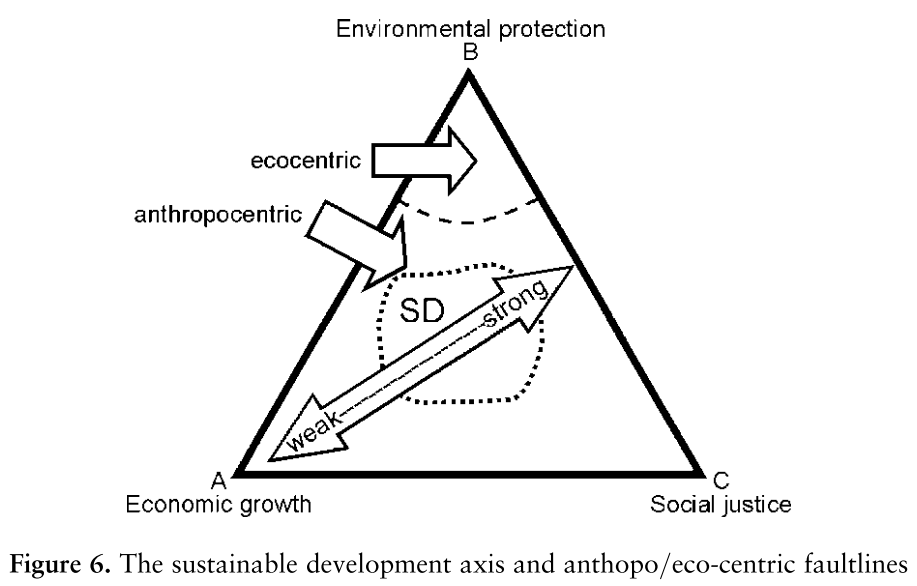
\includegraphics[width=0.5\textwidth]{sections/asset/contested.PNG}
    \caption{Sustainability concept mapped}
    \label{fig:sustainable_map}
\end{figure}


In a similar note, \textcite{Campbell1996} \textbf{Which other authors?} scrutinized the concept of sustainability and specifically asked \textit{'The more practical question is whether sustainability is a useful concept for planners'}. According to him the answer here was mixed, he continues \textit{'(...) We also might be able to define sustainability yet be unable ever to actually measure it or even know, one day in the future, that we had achieved it. An old eastern proverb identifies the western confusion of believing that to name something is to know it. That may be the danger in automatically embracing sustainable development: a facile confidence that by adding the term “sustainable” to all our existing planning documents and tools (sustainable zoning, sustainable economic development, sustain- able transportation planning), we are doing sustainable planning. Conversely, one can do much beneficial environmental work without ever devoting explicit attention to the concept of sustainability.'}\par

\begin{figure}[h!]
    \centering
    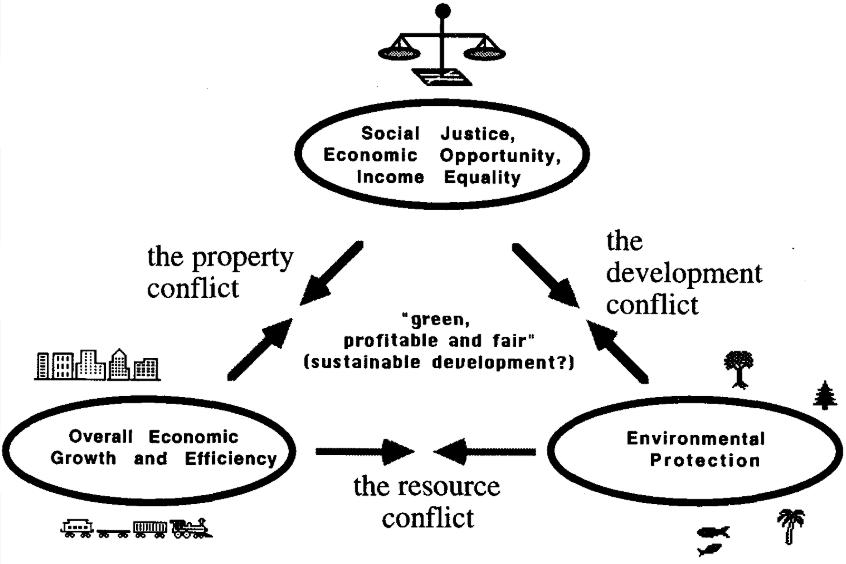
\includegraphics[width=0.5\textwidth]{sections/asset/sdg_conflicts.PNG}
    \caption{conflict triangle of circles}
    \label{fig:sustainable_conflicts}
\end{figure}


In his research, one of the two main procedural avenues to sustainable development suggests to \textit{'redefine the language of the conflict'}. Besides dealing with translation problems, he suggests that these bilingual translations would be extended to the empirical level. Meaning that planners need to find the way to integrate infrastructure, social, economical and environmental information using \textbf{Geographic Information Systems (GIS)}. \par
Besides this strategy, he also recognizes that sustainability should also be pursued in a more traditional way: using market mechanisms to link environmental and economical goals.\par

In sum, the concept of sustainability is found powerful to communicate an ideal that tries to envision a compromise between environment-society-economic. However the concept is defined, United Nations has identified a concrete set of indicators to measure progress in different domains of sustainability and with guidance of the New Urban Agenda and other complementary planning tools and documents, local governments and regions are realizing the importance of the role they play in attaining both: local and global sustainability. Following \textcite{Berke2000} sustainable planning is assessed taking into consideration six domains:\par


\begin{enumerate}
    \item Harmony with nature
    \item Livable built environments
    \item Place-based economy
    \item Equity
    \item Polluters pay
    \item Responsible regionalism
\end{enumerate}

The examination of 30 Comprehensive Urban Plans reveled that there is no correlation between including the term sustainability and how is actually implemented. Among the possible causes they found that in some cases planning agencies lack the competences or sufficient knowledge to steer policies in the right direction. This is also found in  \textbf{make the proper references} while investigating how the SDGS and the NUA were using by planning professionals in Europe. Among the recommendations to overcome this, \textcite{Berke2000} suggest that more research is needed to establish the link between plans, implementations and outcomes. This will be achieved by bridging the gap between the theoretical concepts of sustainability and practices, which indicates a need to provide instruments of planning and measuring the practical outcomes in the territory.\par 

In recent years, the concept of CE has been identified by the private and public sector as an effective strategy/concept/paradigm to achieve several sustainable goals. In the light of such momentum, scholars started to pay attention to the concept and interpellate what does it mean, how effective is it and how to measure this new conceptual framework. \par

%%%%%%%%%%%%%%%%%%%%%%%%%%%%%%%%%%%%%%%%%%%%%%%%%%%%%%%%%%%%%%
\subsection{Circular Economy}
%%%%%%%%%%%%%%%%%%%%%%%%%%%%%%%%%%%%%%%%%%%%%%%%%%%%%%%%%%%%%%%%%
•	[On the origins of CE] \par
\parencite{Prieto-Sandoval2018}


•	[About the concept] \par  
\parencite{Kirchherr2017} 114 definitions of circular economy



\parencite{Korhonen2018a}
Circular economy (CE) is a concept currently promoted by the EU, by several national governments including China, Japan, UK, France, Canada, The Netherlands, Sweden and Finland as well as by several businesses around the world. The European Commission recently esti- mated that circular economy-type economic transitions can create 600 billion euros annual economic gains for the EU manufacturing sector alone (COM, 2014; EMAF, 2013;see also CIRAIG, 2015 and COM, 2015). Finland's Independence Celebration Fund (FICF, SITRA) and Mckinsey (2014) jointly estimate 2.5 billion euros annual gains for the national economy of Finland through circular economy. The global economy would benefit 1000 billion US dollars annually (FICF and Mckinsey, 2014;see e.g. EMAF, 2013). China, as the first country in the world, adopted a law for the circular economy in 2008 (CIRAIG, 2015). Circular economy is recommended as an approach to economic growth that is in line with sustainable environmental and economic develop- ment (see EMAF et al., 2015; EMAF, 2013; EMAF, 2012; CIRAIG, 2015; COM, 2015; COM, 2014).


The scientific and research basis of the CE approach seems to be only in its infancy. To authors' knowledge the definition given above in section three (3) is the first attempt to present a scientific research-based definition of CE. Many key questions are still open. These will arise, e.g. from the nature of self-organized complex social-ecological systems (see e.g., Chertowand Ehrenfeld, 2012; Folke, 2006) to which CE systems belong.



•	[CE as a paradigm change?] \par 
 \parencite{Geissdoerfer2017}

•	[Where are we standing in terms of the concept and its maturity] \par
\parencite{Blomsma2017}

Using the umbrella concept in \textcite{Blomsma2017} conclude that whereas the various resource strategies grouped under the CE’s banner are not new individually, the concept offers a new framing of these strategies by drawing attention to their capacity of prolonging resource use as well as to the relationship between these strategies. As such, the CE offers a new perspective on waste and resource management and provides a new cognitive unit and discursive space for debate. 
Hirsch and Levin (1999) define an umbrella concept as: “a broad concept or idea used loosely to encompass and account for a set of diverse phenomena” (Hirsch and Levin (1999), 200). Umbrella concepts create a relation between pre-existing concepts that were previously unrelated, or not related in the manner the umbrella concept proposes, by focusing the attention on a particular shared quality or characteristic of the concepts it encompasses.


\begin{figure}[h!]
    \centering
    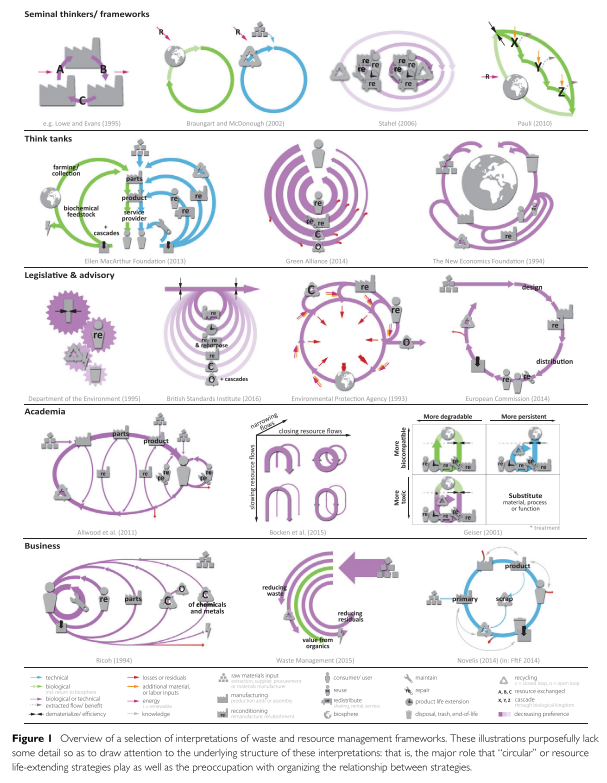
\includegraphics[width=0.5\textwidth]{sections/asset/ce_frameworks.PNG}
    \caption{Sustainability concept mapped}
    \label{fig:sustainable_map}
\end{figure}



\begin{figure}[h!]
    \centering
    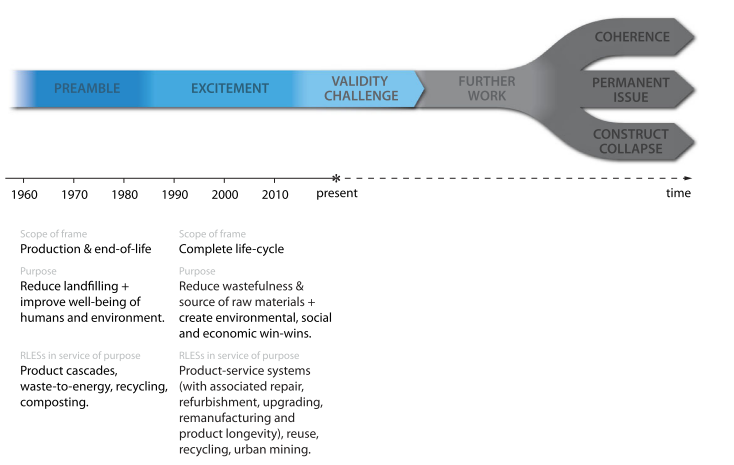
\includegraphics[width=0.5\textwidth]{sections/asset/ce_fork.PNG}
    \caption{CE concept trajectory}
    \label{fig:ce_path}
\end{figure}





•	[Also an essentially contested concept] \par
\parencite{Korhonen2018}

•	[Umbrella concept] \par

\parencite{Homrich2018}

•	[Relevance to SDG] \par

In relation to better resource management and minimize the the damage to the environment the concept/paradigm/strategy of Circular Economy has gained momentum as a possible path to directly incidence in SDG numbers 7-8, 12, 6 \& 15 
\parencite{Schroeder2018}

\begin{figure}[h!]
    \centering
    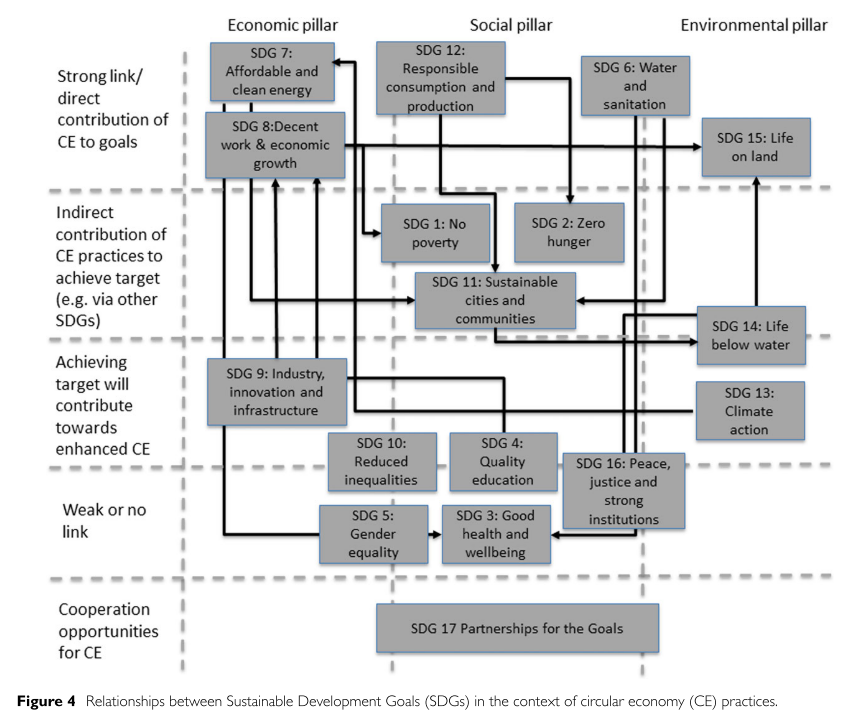
\includegraphics[width=0.5\textwidth]{sections/asset/ce_relation.PNG}
    \caption{Contribution of CE to SDGs}
    \label{fig:sustainable_conflicts}
\end{figure}


•	[However, it seems to be a clear productivity incentive behind] \par
increase in productivity of firms \parencite{Moric2020}:
Our analysis of more than 4000 SMEs from 28 EU Member States suggests that the implementation
of practices related to the circular economy positively influences productivity, which supports our first hypothesis. This finding is consistent with the argument that the investment in the circular economy generates, along with environmental benefits, economic ones through resource use and waste minimisation [7,8,13–17]


•	[Also questions of how achievable is it and why we want to close resource loops locally?]

\parencite{Gregson2015}
The concept of the circular economy has gained increasing prominence in academic, practitioner and policy circles and is linked to greening economies and sustainable development. However, the idea is more often celebrated than critically interrogated. Analysis shows the concept circulates as an idea and ideal, exemplified by industrial symbiosis and extended product life. Yet, its actual enactment is limited and fragile. Instead, circular economies are achieved mostly through global recycling networks which are the primary means by which wastes are recovered as resources. European policies eschew these circuits. Resource recovery through global recycling networks is regarded as a dirty and illegal trade. In its place, EU circular economies attempt to transform wastes into resources within the boundaries of the EU. Through an analysis of two case studies of resource recovery in the United Kingdom, we highlight the challenges that confront making circular economies within the EU, showing that these are borne of a conjuncture of politically created markets, material properties and morally defined materials circuits. We show resource recovery in the EU to be framed by moral economies, driven by discourses of ecological modernization environmental justice and resource (in)security, the last of which connects to China’s resource-intensive development.

•	[what type of research is done] \par
\parencite{Merli2018} scholars approaching to circular economy concept



•	[Barriers to Circular Economy] \par 


•	[Overcoming barriers with digital tools] \par \parencite{Okorie}\par

\parencite{Amato2019}
Our results suggest that the use of eco-information sources and trust in different providers significantly affect green behaviors of EU citizens towards a ‘truly’ circular economic system








•	[Example of industry 4.0 in Italian case study] \par \parencite{Economy}



%%%%%%%%%%%%%%%%%%%%%%%%%%%%%%%%%%%%%%%%%%%%%%%%%%
\subsubsection{Urban Metabolism}
%%%%%%%%%%%%%%%%%%%%%%%%%%%%%%%%%%%%%%%%%%%%%%%%%%


Urban metabolism approach to manage cities \parencite{Kalmykova2015}

%\subsubsection{Solid Waste Management System}




%%%%%%%%%%%%%%%%%%%%%%%%%%%%%%%%%%%%%%%%%%%%%%%%%%%%
\subsubsection{Industrial Ecology}
%%%%%%%%%%%%%%%%%%%%%%%%%%%%%%%%%%%%%%%%%%%%%%%%%%%%%%%
•	[The origins of the concept] \par
\parencite{Jelinski1992}\par


•	[on industrial symbiosis theory and practice:] \parencite{Zhang2015a} \par

•	[Contribution of Industrial Ecology to Circular Economy] \par \parencite{Saavedra2018} \par

•	[Change in paradigm?] \parencite{Ehrenfeld2000} \par

•	[Industry 4.0 and industrial symbiosis] \par
\parencite{Tseng2018}\par


•	[Explaining Industrial Symbiosis Emergence, Development, and Disruption]\par \parencite{Yap2017}\par




% %%%%%%%%%%%%%%%%%%%%%%%%%%%%%%%%%%%%%%%%%%%%%%%%%%
% \subsubsection{Summary}
% %%%%%%%%%%%%%%%%%%%%%%%%%%%%%%%%%%%%%%%%%%%%%%%%%%
% Along this 



% The concept and research is at an infant stage and the lack of a proper operational definition makes it and Essentially Contested Concept \parencite{Korhonen2018}. 

% 'However, the CE approach has almost exclusively been developed and led by practitioners, i.e., policy-makers and business development agencies such as business consultants, business associations, business foundations etc. (e.g., EMAF, 2013; COM, 2014; CIRAIG, 2015). From a scholarly position, the conceptual discussions on CE are still in their infancy and the literature is only emerging.'

% After the review, a proposal of the definition is made.

% 'CE is a sustainable development initiative with the objective of reducing the societal production-consumption systems' linear material and energy throughput flows by applying materials cycles, renewable and cascade-type energy flows to the linear system. CE promotes high value material cycles alongside more traditional recycling and develops systems approaches to the cooperation of producers, consumers and other societal actors in sustainable development work.' 




%%%%%%%%%%%%%%%%%%%%%%%%%%%%%%%%%%%%%%%%%%%%%%%%%%
\section{Urban \& regional science (URS)}
%%%%%%%%%%%%%%%%%%%%%%%%%%%%%%%%%%%%%%%%%%%%%%%%%%

His agricultural landuse model forms the foundation for all urban land models today. Von Thunen’s goal was to answer the question, “I have a piece of land, what is the best use for that land?”
In 1885, mathematician Carl Wilhelm Friedrich Launhardt pioneered the relation between land use and land rents in what are called “bid-rent functions.” He also explored the concept of market area analysis and spatial demand curves. Alfred Weber’s Theory of Industrial Location followed Thunen’s example by asking: “I have an industry, where do I locate it?” 
Walter Christaller developed a model showing how cities are linked in a hierarchical network in his 1933 work, Central Places in Southern Germany. Finally, in 1944 August Losch expanded on this network with his work Die The Economics of Location, where he developed a formal model of market areas to complement Christaller’s system of cities.


Starting in this chapter, we relax the assumption that resources are equally distributed over a homogeneous plain. We assume pockets of dense population, as well as immovable resources such as lakes, rivers, mountains, forests, and coal mines. In this chapter, we will study several models of least-cost location. First, we will investigate what a least-cost location entails. Because firms can substitute various quantities of each input for one another, finding a least-cost location involves more than a comparison of the cost of inputs at different potential sites. As the example of Urban Center and Pine Grove illustrates, firms will use different proportions of inputs depending on their costs at various locations. Second, a firm’s cost structure depends on its size. The concept of increasing returns to scale is vital in explaining where economic activity locates, so we will examine the influence of internal economies of scale on location choice. Third, from the transportation models, we discovered that there are a limited number of potential locations that can minimize total costs. Firms might decrease total transportation costs by bringing inputs to the plant and selling the product locally. Instead, they may consider shipping their output to a distant market and locating close to their inputs. To see the distinction, we to examine Hoover’s (1971) theories of how transportation influences manufacturing firm location.



% \begin{figure}[h!]
%     \centering
%     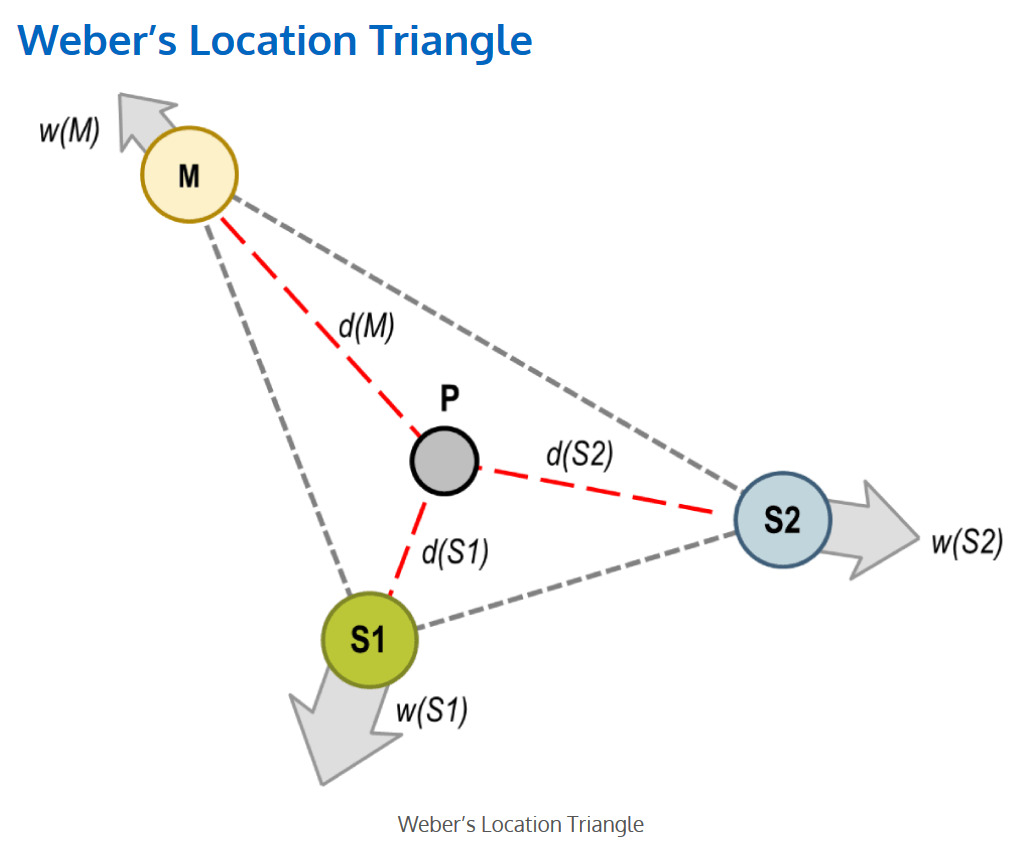
\includegraphics[width=0.4\textwidth]{sections/asset/weber.PNG}
%     \caption{Industrial location}
%     \label{fig:weber}
% \end{figure}

Weber....

\begin{figure}[h!]
    \centering
    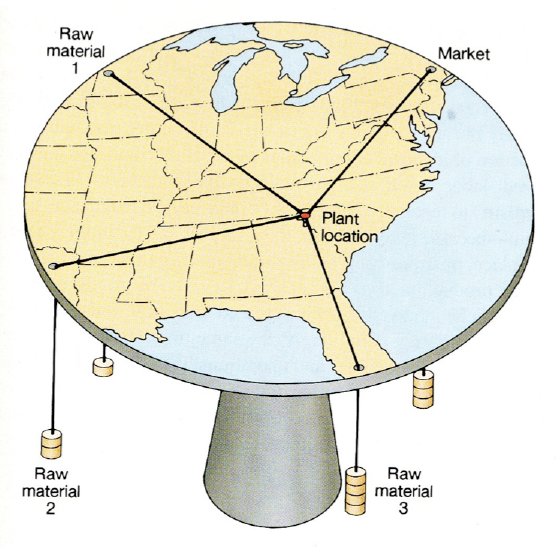
\includegraphics[width=0.4\textwidth]{sections/asset/weber1.PNG}
    \caption{Industrial location old school}
    \label{fig:weber}
\end{figure}


%%%%%%%%%%%%%%%%%%%%%%%%%%%%%%%%%%%%%%%%%%%%%%%%%%
\subsection{Economic growth of regions}
%%%%%%%%%%%%%%%%%%%%%%%%%%%%%%%%%%%%%%%%%%%%%%%%%%

In recent research in economic geography, an empirical body of literature has emerged on the role of related variety in regional development. The concept of related variety was put forward by \textbf{Frenken et al. (2007) }as to further specify the common hypothesis that regions benefit from producing a variety of products and services, as more variety implies more potential for inter-industry knowledge spillovers. \textbf{Frenken et al. (2007)} emphasized that: “one expects knowledge spillovers within the region to occur primarily among related sectors, and only to a limited extent among unrelated sectors” (p. 688). That is, they hypothesized that inter-industry spillovers occur mainly between sectors that draw on similar knowledge: knowledge originating from one sector is most relevant to, and can most effectively be absorbed by, another sector that is related in the sense that firms draw on similar knowledge (about technology, markets, etc.).
The concept of related variety was introduced in an attempt to resolve an earlier empirical question put forward by \textbf{Glaeser et al. (1992)} whether regions benefit most from being specialized or being diversified. This "controversy" is commonly referred to as MAR versus Jacobs referring to the theories of \textbf{Marshall, Arrow and Romer suggesting spillovers} to take place primarily within a single industry versus the theory of \textbf{Jacobs (1969, p. 59) }who argued that “the greater the sheer numbers and varieties of divisions of labor already achieved in an economy, the greater the economy’s inherent capacity for adding still more kinds of goods and services". The theories of MAR view innovation mainly as incremental where firms learn from knowledge and innovation from same-industry firms (otherwise known as "localization economies"), while Jacobs views innovation essentially as a recombinant process that necessarily builds on a pre-existing variety of knowledge and artefacts that are being combined in new ways leading to new products and services, viz. new employment.



The concept of related variety is consonant with the concept of \textbf{product space} introduced by \textbf{Hidalgo et al. (2007).} They argued that countries develop by diversifying their export portfolio over time. They showed that countries typically do so by “branching out”, that is, by entering export products that are closely related to the products they already export. The reasoning underlying this phenomenon holds that once a country has developed the capabilities to specialize in exporting particular products, it can easily diversify in related products that require very similar capabilities to produce them. By calculating, for each possible new product, the “density” of related products already present in a country’s export portfolio, the authors could show that the higher the density of related products vis-à-vis a potential new product, the higher the chance that a country will diversify into this new product. This idea is in line with related variety, because the more products a country already exports related to a product that it does not yet export, the more likely you will start exporting that product as well in the future. The difference between the related-variety and the product density concepts is that the former is use to explain aggregate employment growth while the latter is used to explain diversification events into new products.



•	[Space was poorly considered]\par 



%%%%%%%%%%%%%%%%%%%%%%%%%%%%%%%%%%%%%%%%%%%%%%%%%%
\subsection{How Regions functions - what is a function}
%%%%%%%%%%%%%%%%%%%%%%%%%%%%%%%%%%%%%%%%%%%%%%%%%%
 sectors
 wages
 international trade
 


% %%%%%%%%%%%%%%%%%%%%%%%%%%%%%%%%%%%%%%%%%%%%%%%%%%
% \subsection{Structuralist - Economic theory from Marx to Smith}
% %%%%%%%%%%%%%%%%%%%%%%%%%%%%%%%%%%%%%%%%%%%%%%%%%%


%%%%%%%%%%%%%%%%%%%%%%%%%%%%%%%%%%%%%%%%%%%%%%%%%%
\subsection{New Economic Geography}
%%%%%%%%%%%%%%%%%%%%%%%%%%%%%%%%%%%%%%%%%%%%%%%%%%
Inspired by the New Economic Geography (NEG) approach, initiated by \textbf{Paul Krugman and Masahita Fujita} in the 1990s, the main objective of the COST Action 1104 “The EU in the new complex geography of economic systems: models, tools and policy evaluation (GeComplexity)” has been to approach the study of EU, more generally, economic systems from a multi-layered perspective featuring interconnected spatial structures. At each layer, different types of decisions and interactions take place: interactions among international or regional trading partners at the macro-level; the functioning of (financial, labour) markets as social network structures at the meso-level; and finally, the strategic choices of single firms and households at the micro-level. Within these structures, the spatial distribution of economic activities is evolving through time following complex patterns determined by economic, geographical, institutional and social factors. To study these structures, during its four years life time (March 2012–September 2016), the Action has built successfully an interdisciplinary approach. It has further developed advanced mathematical, computational and empirical methods and tools for analysing complex nonlinear systems, including macro and micro models, nonlinear dynamical systems, social networks, game theoretical models and agent based models.



%%%%%%%%%%%%%%%%%%%%%%%%%%%%%%%%%%%%%%%%%%%%%%%%%%
\section{Urban \& regional planning}
%%%%%%%%%%%%%%%%%%%%%%%%%%%%%%%%%%%%%%%%%%%%%%%%%%


\parencite{WongTai-Chee;YuenBelinda;Goldblum2008}


Indeed, the concern with sustainable urban development arises and takes place in a world of economic globalization and of technological revolution, a world where the financial market’s selective expansion and innovation in the realm of communications systems has benefited strategic urban locations specifically catalytic to economic growth. Cities having built up a silent but revolutionary capacity in mastering flows (goods, people and information), in terms of paths and speed could affect their position and functions, their scale and ability in coping with these issues. If the rise of ecological ideas and consciousness in the early 1970s has been associated with “zero economic growth” (a concept promoted by the Club of Rome during the first oil crisis) and with the ideals of small/local dimensions (Schumacher 1973), the relationship between global dynamics and local development as expressed by the notion of “glocalism” are associated with mega-urban dimensions. The processes leading to this new representation of urban growth, the way to master its effects at urban, territorial and world scales, and to match it with the ideal of “sustainable development” naturally question the significance and the very nature of urban planning.\par

The objective of spatial planning for sustainability is primarily to counter the adverse effects of urban developments by means of systematic and organized land use planning activities. Sustainability planning has a holistic outlook which calls for an integration of the goals of the three Es (Economic, Environmental and Equity concerns) into an organized coherent system for a long-term objective formulation and plan implementation. No country can or should conduct sustainability planning in isolation, as the “stretching and deepening of global-scale processes” has exerted intricate interaction and reaction in one way or another on local scales (see Olds 2001: 19).\par



In terms of objectives, planning was no more dedicated to solving urban problems (in the sense of a corrective urbanism), but as a way to rationalize the city machinery itself, and to make it an efficient engine for nation-building and economic development.  




%%%%%%%%%%%%%%%%%%%%%%%%%%%%%%%%%%%%%%%%%%%%%%%%%%
•	[Why do planning theory?: theory-practice gap]
%%%%%%%%%%%%%%%%%%%%%%%%%%%%%%%%%%%%%%%%%%%%%%%%%%
[\parencite{Yiftachel1989}] \par
[\parencite{Alexander2003}] \par
[\parencite{Alexander1997}] \par
[\parencite{Friedmann2003}] \par





In another note, \parencite{Campbell1996}, envisioned that 

\textit{The role of the planner in all four of these approaches is to arrange the procedures for making decisions, not to set the substance of the actual outcomes. In some cases, the overall structure for decision- making already exists (the market and the political system). In other cases, however, the planner must help shape that structure (a mediation forum; a common language), which, done successfully, gives the process credibility. The actual environmental outcomes nevertheless remain unknowable: you don’t know in advance if the environment will actually be improved.
}


\parencite{Friedmann1993}
'But what we are living through in the final decades of this century (1993) is something altogether different. It is nothing less than the collapse of the Euclidean world order of stable entities and common sense assumptions that have governed our understanding of the world for the past two hundred years.'
'We are moving into a non-Euclidean world of many space-time geographies, and it is the recognition of this change that obliges us to think of new and more appropriate models.'\par

[DEFINITION OF PLANNING]:
Planning is that professional practice that specifically seeks to connect forms of knowledge with forms of action in the public domain.'\par

'(...) we need first to consider the implications of the contemporary collapse of the time-space continuum. What would be the appropriate time and space of a non-Euclidean form of planning? The time of such planning is the \textit{real time} of everyday events rather than imagined future time.'\par

'Viewed in this light, planning becomes less a way of preparing documents, such as analyses and plans, and more a way of bridging planning knowledge and practice to bear directly on the action itself.'\par

'Concern with an imagined future will continue to play an important role in planning, but the emphasis in non-Euclidean planning should be on processes operating in actual or real time, because it is only in the evanescent and still undecided present that planners can hope to be effective.'\par

'As for the space of planning, we need to privilege \textit{regional and local} over national and transnational planning. This leads to a decentered view of planning 
-> 1. Heterogeneity of local places \par
-> 2. Organized civil society \par
-> 3. Regions and localities are the spaces of people's everyday lives. National and transnational space is typically for corporate actions and super ordinate bureaucracies.\par






\parencite{Casella2007}
'I have no quarrel with Friedmann’s characterization
of the non-Euclidian planning model as normative, innovative, political, transactive, and based on social learning. Those characteristics are validated by my own experience. But, I would add four other characteristics to Friedmann’s five, and call it a quantum model. A quantum planning model would also be technological, multidisciplinary, substantive, and intellectually free:'






%%%%%%%%%%%%%%%%%%%%%%%%%%%%%%%%%%%%%%%%%%%%%%%%%%
\subsubsection{Circular cities}
%%%%%%%%%%%%%%%%%%%%%%%%%%%%%%%%%%%%%%%%%%%%%%%%%%



\begin{figure}[h!]
    \centering
    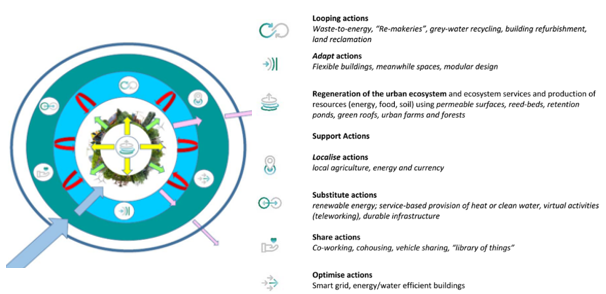
\includegraphics[width=0.8\textwidth]{sections/asset/city.PNG}
    \caption{Circular cities}
    \label{fig:research objectives}
\end{figure}






%%%%%%%%%%%%%%%%%%%%%%%%%%%%%%%%%%%%%%%%%%%%%%%%%%
\subsubsection{GIS, Geodesing and Spatial Decision Support Systems (SDSS)}
%%%%%%%%%%%%%%%%%%%%%%%%%%%%%%%%%%%%%%%%%%%%%%%%%%


\parencite{Anselin1993}

% \begin{figure}[h!]
%     \centering
%     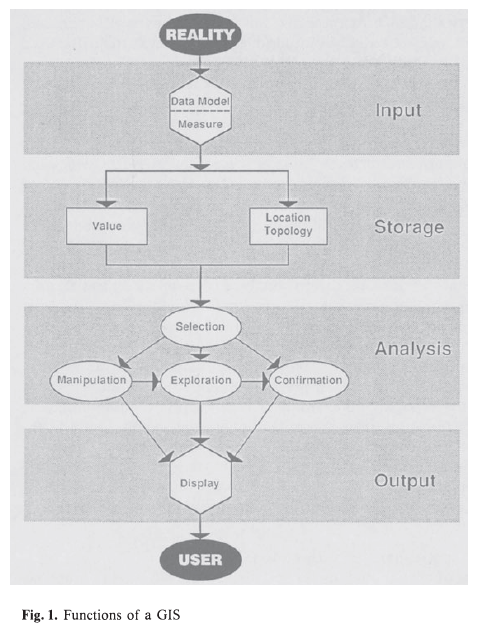
\includegraphics[width=0.2\textwidth]{sections/asset/anslein.PNG}
%     \caption{GIS framework}
%     \label{fig:anselin}
% \end{figure}




%%%%%%%%%%%%%%%%%%%%%%%%%%%%%%%%%%%%%%%%%%%%%%%%%%
\subsubsection{Urban analytics}
%%%%%%%%%%%%%%%%%%%%%%%%%%%%%%%%%%%%%%%%%%%%%%%%%%
Different approaches have been used to address all sort of urban problems. Ranging from case studies, ethnography to more quantitative methods such as mathematical modelling or statistical verification of hypothesis. 
Urban Analytics and Informatics is a relatively new, multidisciplinary, and broad field of research that also contributes to identify, describe and solve urban challenges. Its name indicates the conjunction of two disciplines. On one hand, brings specific knowledge from economics, sociology, or geography to address urban dynamics such as gentrification, segregation, lack of accessibility or housing informality. On the other hand, uses a quantitative approach to understand these dynamics. Urban analytics focuses on many domains but uses a specific toolbox to explore these topics. \par
Michael Batty, founder of the Center of Advanced Spatial Analytics (CASA) at UCL defines it as a \textit{`fast emerging as the core set of tools employed to deal with problems of big data, urban simulation, and geodemographics'} and Michael Goodchild states that is a \textit{`New kind of urban research, one that exploits the vast new data resources that are becoming available from social media, crowd sourcing, and sensor networks (...)'}\parencite{singletonUrbanAnalytics2018}. \par
\begin{figure}[h!]
    \centering
    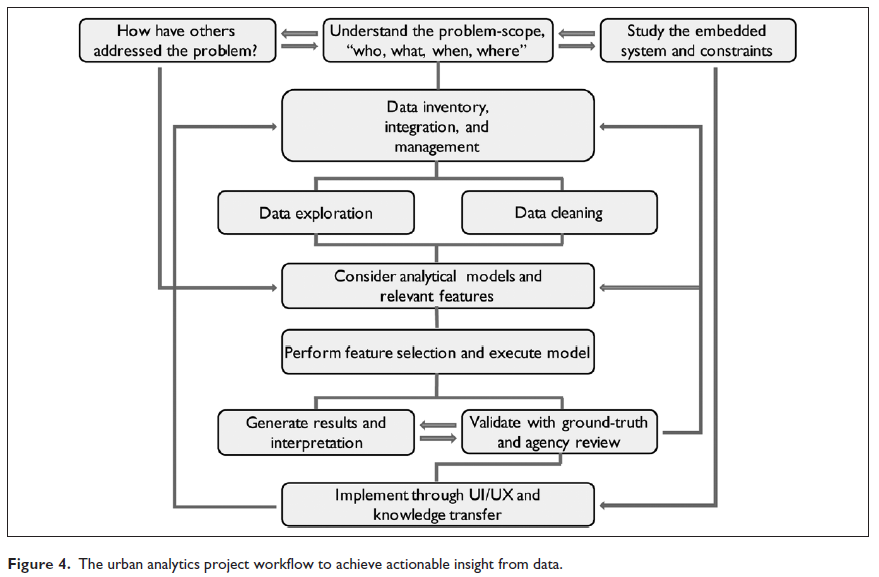
\includegraphics[width=0.9\textwidth]{sections/asset/data.PNG}
    \caption{Urban analytics}
    \label{fig:urbandata}
\end{figure}


During recent years, a set of new forms of data and computational approaches have enabled a new science of cities to rise \parencite{battyNewScienceCities2013}. But as the old KPIs, these new data sources do not produce insights on their own. Data needs to be stored, cleaned and combined with different sources to be used. Urban Analytics is the disruptive approach that enables to handle big quantities of information to answer urban questions. Among the toolbox often employed we could list: (i) Modelling, (ii) Visualization, (iii) Data Capture, (iv) Data Science, (v) GIS and (vi) Simulations. \par

In order to illustrate what Urban Analytics and Informatics is capable of, a set of four projects are described below. Although, in each project different features of the toolkit are used, the strongest and most innovative resource was highlighted: 



\begin{enumerate}


    \item{Data Science}
In this case (Figure \ref{fig:ds}), Treepedia \footnote{\url{http://senseable.mit.edu/treepedia}} Google Street View is used to create a perception index of how green a city is. In opposition to using satellite images or tree census, the objective of this project is to capture the amount of perceived green by the citizens of a settlement. Besides the innovative use of an already existing data source, the project is data intensive, as the images need to be processed and determine the amount of greenery.



    \item{New Data Sources}
The second case (Figure \ref{fig:nds}), is named Tasty Data and\footnote{\url{http://senseable.mit.edu/tasty-data/}} tries to tackle one of the mayor data limitations faced by planners, politicians or any other stakeholder of the city. Using the data of a food service application the project managed to estimate the amount of people that lived in different cities in china. The results produced a more detailed dataset of the population (temporal and spatial) than what an official census can provide.


    \item{Data Capture}
In some cases , Urban Analytics and Informatics can contribute to create a new data set. In this case 9Figure \ref{fig:dc}), the project is known by Trash Track \footnote{\url{http://senseable.mit.edu/trashtrack/}} and a  small trackable devices are embedded in objects to be thrown away. As a result, the, spatial-temporal trace of waste is generated. There is a completely new data set of where the waste is generated, where did it traveled and for how long and where it ended. 




    \item {Visualizations}
Another important component of Urban Analytics is to summarize the findings and highlights of big and complex data sets in a comprehensible way. Using an adequate visual strategy is important to make the results of the research understandable by a specific audience. In this case (Figure \ref{fig:viz}), GeoFluxus\footnote{\url{http://geofluxus.com/##data}}, was selected as an example as the project objective is to map and visualize the flow of waste.


\end{enumerate}

\begin{figure}[H]
    \begin{multicols}{2}
    \noindent
    \subfloat[Data Science\label{fig:ds}]{\centering
    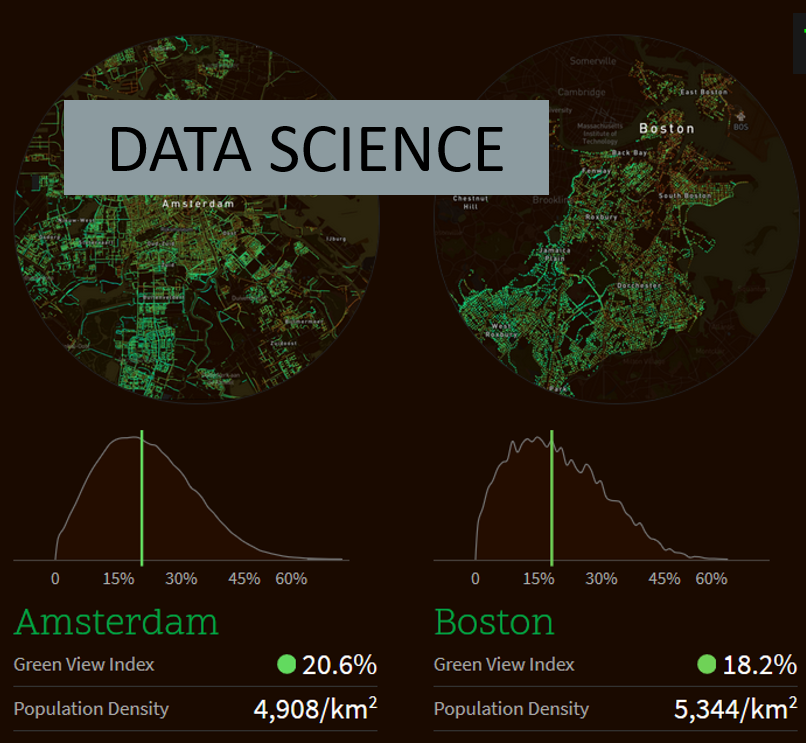
\includegraphics[width=0.9\linewidth, height=6cm]{sections/asset/4_ds.PNG}}
     
    %
    \subfloat[New Data Sources\label{fig:nds}]{\centering
    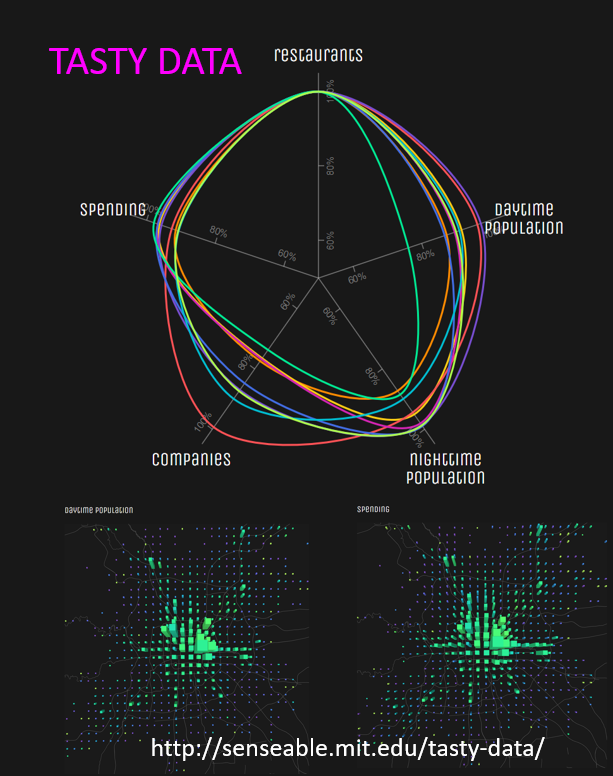
\includegraphics[width=0.9\linewidth,height=6cm]{sections/asset/5_new_data.PNG}}\newpage
    %
    \subfloat[Data Capture\label{fig:dc}]{\centering
    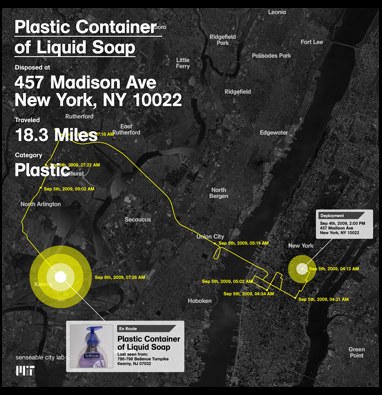
\includegraphics[width=0.9\linewidth,height=6cm]{sections/asset/6_trash_track.PNG}}\par
    %
    \subfloat[Visualization\label{fig:viz}]{\centering
    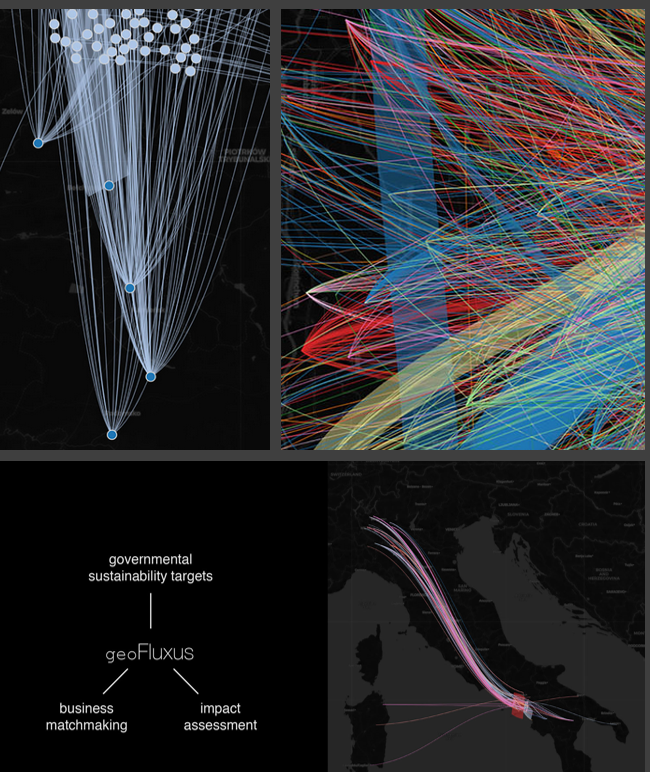
\includegraphics[width=0.9\linewidth, height=6cm]{sections/asset/7_flux.PNG}}
    %
    \end{multicols}
    \caption{Examples of Urban Analytics and Informatics toolkit}
    \label{UA_toolkit}
\end{figure}



% %%%%%%%%%%%%%%%%%%%%%%%%%%%%%%%%%%%%%%%%%%%%%%%%%%%%%%
% \section{Related work} 
% %%%%%%%%%%%%%%%%%%%%%%%%%%%%%%%%%%%%%%%%%%%%%%%%%%%%%%
% Maybe a different chapter




